\textbf{Question 13.} \\
\hrule 

A computer consulting firm presently has bids out on three projects. Though the book refers to awarded projects using $A_i$, let us instead use $A, B$ and $C$ for the respective three rewards to improve readability. Suppose that $P(A) = .22$, $P(B) = .25$, $P(C) = .28$, $P(A \cap B) = .11$, $P(A \cap C) = .05$, $P(B \cap C) = .07$, $P(A \cap B \cap C) = .01$. Express in words the following events, and compute the probability of each event. 
\begin{align*}
    P(A) &= .22 \\ 
    P(B) &= .25 \\ 
    P(C) &= .28 \\
    P(A \cap B) &= .11 \\
    P(A \cap C) &= .05 \\
    P(B \cap C) &= .07 \\ 
    P(A \cap B \cap C) &= .01
\end{align*}

Using this given information I was able to construct this Venn diagram. \newline
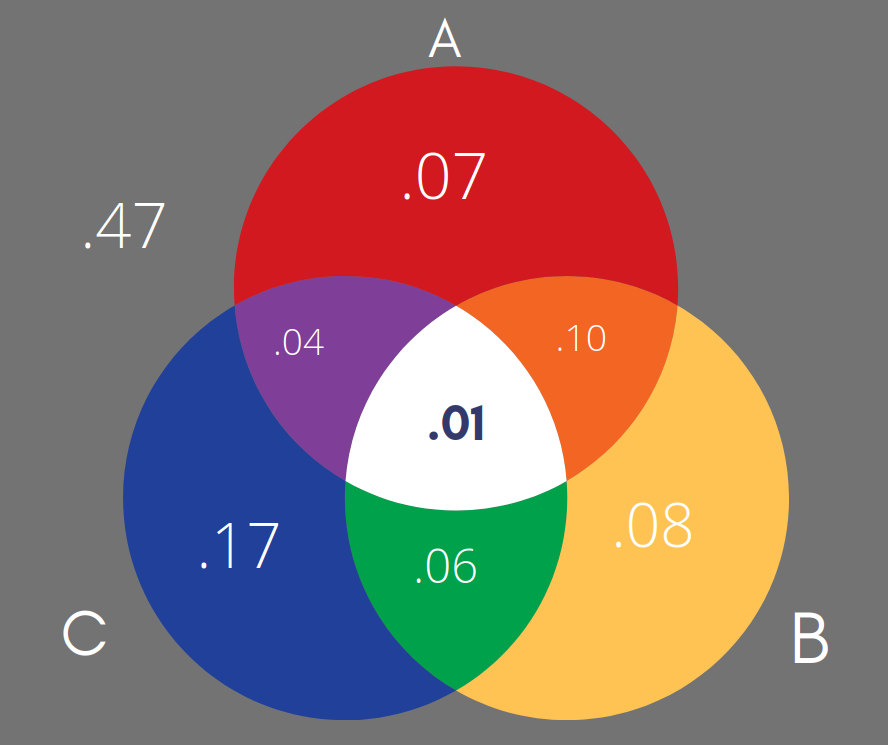
\includegraphics[scale=0.25]{images/whw3/2.2.13_venn.png}

\textbf{a.} $A \cup B$ \newline 
This event would be when either project A or project B gets an award. \newline 
$P(A \cup B) = 0.07 + 0.10 + 0.01 + 0.08 + 0.06 = 0.32$

\textbf{b.} $A' \cap B'$ \newline 
This event is the intersection of not A and not B. To break this down. Not A involves the yellow, green, blue and grey sections. Not B involves the blue, purple, red and grey sections. The intersection here is what is in both of these sets. That is, blue and grey. So, this event is when either only Project C gets an award, or none of the projects get an award. \newline 
$P(A' \cap B') = .47 + .17 = 0.64$

\textbf{c.} $A \cup B \cup C$ \newline 
This event is any of the three projects getting an award. It encompasses the whole interior of the Venn diagram. As such: $P(A \cup B \cup C) = 1 - .47 = .53$

\textbf{d.} $A' \cap B' \cap C'$ \newline 
This event is none of the three projects getting an award. It is the outside portion of the Venn diagram. As such, $P(A' \cap B' \cap C') = .47$

\textbf{e.} $A' \cap B' \cap C$ \newline
This event is neither A or B getting an award, but C getting an award. It is only the blue section of the Venn diagram. $P(A' \cap B' \cap C) = .17$

\textbf{f.} $(A' \cap B') \cup C$ \newline 
This event is two parts. The first is the intersection of not A and not B, which is still blue and grey as discovered in part b. We then get the union of that with C, which gives us blue, green, white and purple. So we get the following probability. \newline 
$P((A' \cap B') \cup C) = .47 + .17 + .04 + .01 + .06 = .75$ \newline 
\hrule 